\documentclass[a4paper,12pt]{article}
\usepackage{fontspec}
\setmainfont{Times New Roman}
\usepackage[a4paper,left=5mm,right=5mm,bottom=5mm,top=5mm]{geometry}
\usepackage{hyperref}
\usepackage{url}
\usepackage{float}
\usepackage{subcaption}
\usepackage{amsmath}
\usepackage{graphicx}
\usepackage{color}
\usepackage[style=numeric]{biblatex}
\addbibresource{references.bib}
\usepackage{multirow}
\usepackage{makecell}
% \usepackage{xcolor} 
% \pagecolor[rgb]{0.12,0.12,0.12} 
% \color[rgb]{1,1,1}
\usepackage[table,xcdraw]{xcolor}

\begin{document}

\title{Completely Contactless and Online Finger Knuckle Identification}
\author{Zhenyu ZHOU}
\maketitle

\setlength{\parindent}{0em}
\setlength{\parskip}{0.5em}

\input{FK-Identification/abstract.tex}
\section{Introduction}

Biometrics is the use of the human body's inherent physiological and behavioral characteristics for person identification. For the physiological characteristics, there are many human characteristics such as retina, iris, face, fingerprints and palm prints; as far as the behavioral characteristics, the available features include gait recognition, voice and other behavioral characteristics. As for the finger knuckle, it has also attracted many researchers devoted to it, because it is easier to expose, easier to collect, and it has also been proven to be unique and stable \cite{kumar2014importance}. Many early works on biometric recognition of finger knuckle, ranging from coding-based methods, subspace methods and texture analysis methods to 3D shape patterns based on 3D image reconstruction, and different methods have been used to achieve highly accurate recognition results. 

Contactless finger knuckle identification should be studied extensively because it is more security and more hygienic, especially now with COVID-19. At the same time, It has attracted the attention of many researchers and achieved many result. Even early work considered application scenario using cell phones for finger knuckle recognition \cite{cheng2012contactless}, but for finger knuckle segmentation using fixed finger position in the centre of the image is not very convenient for the user, for recognition phase log-Gabor is used for feature extraction, and Hamming distance is used for matching. Meanwhile these paper \cite{kumar2019toward}, \cite{cheng2020deep}, \cite{kapoor2020completely} are the latest in research on the topic.

\subsection{Related Work}
\textbf{Finger Knuckle Recognition}

For the traditional recognition algorithms, there are generally two main types: one is holistic-based, and the other is local feature-based. The broad category can be divided into subspace and spectral representation methods for holistic-based \cite{yang2011finger}, \cite{neware2013finger}, \cite{meraoumia2011fusion}. Sub-space methods are generally used for data dimensionality reduction and noise reduction \cite{zhang2006biometric}, such as the use of principal component analysis to reduce the dimensionality of multidimensional data. In contrast to spectral representation methods, image space transformation can be performed as well as image feature enhancement and correlation coefficients for feature extraction \cite{hennings2005verification}. For the processing of local information, there are many algorithms, including, for example, extracting information about the gradient of the image edges, obtaining the boundary points, using other edge extraction algorithms such as Hough change. For example, a 1D log-Gabor filter was used to extract the finger knuckles' features and for the matching phase, the hamming distance was used here for the matching score calculation since it is a local feature-based method \cite{meraoumiapersonal}. Alternatively, a 2D Gabor filter is used to extract the domain orientation information features of the finger knuckles, and an angular distance calculation is used to calculate the similarity between the different features for the matching score \cite{mehrotra1992gabor}. High recognition accuracy has been achieved for these matching algorithms, even up to $98.67\%$ \cite{yang2011finger}.

However, these traditional algorithms have a common problem that these algorithms have to keep changing their corresponding filters and even the corresponding detection parameters under different scenario \cite{zheng20163d}. In other words, traditional algorithm cannot learn filters and parameters by themself. With the development of neural network, the generalization ablity of feature extraction and feature matching method becomes more robust. Especially, from the oldest LeNet \cite{lecun1998gradient} to nowadays EfficientNetV2 \cite{tan2021efficientnetv2} model, the CNN models have achieved great success in computer vision tasks. Therefore, the CNN models also can be used on finger knuckle identification tasks. Such as FKNet \cite{cheng2020deep} based on the ResNet-50 \cite{he2016deep}, it use the FKNet to classify the subject from the 3D feature of finger knuckle. There are even manay that combine traditional methods with CNN models. Forr example \cite{kapoor2020completely}, it first extracts different information with Gabor filters, and then uses CNN to learn the most important information.



\textbf{Object Detection and Segmentation}

For the efficiency of the matching algorithm, the accuracy of the region of interest of object is a factor that can determine the matching efficiency and accuray. The size of the region of interest should be comparable to the size of the actual target object at the pixel level so that the size obtained after segmentation will not have redundant pixel information, which will reduce the pixel values to be computed for both the extraction and the subsequent matching sessions. 

As for the traditional method, their \cite{kumar2019toward}, \cite{cheng2012contactless} approach is to fix the finger knuckle position in the image when taking the finger knuckle data without complexity background, and then extract the edges of the object. Most importantly, the traditional segmentation algorithm cannot correctly segment the finger knuckles in the presence of complex background interference, multiple finger knuckles in the same field of view, obscured finger knuckles or bent finger knuckles. It is difficult to use traditional object segmentation methods to automatically segment finger knuckles for applications such as in the wild. Models of neural network models for object detection have achieved great success, whether it is the sliding window detection algorithm, the 2-stage series of R-CNN models \cite{girshick2014rich}, \cite{girshick2015fast}, \cite{ren2015faster}, or the 1-stage YOLO series \cite{redmon2016you}, \cite{redmon2017yolo9000}, \cite{redmon2018yolov3}, \cite{bochkovskiy2020yolov4} and SSD models \cite{liu2016ssd} up to the current position, and even the anchor-free based object detection algorithm \cite{xin2021pafnet} as well. Each of these models has its advantages. For the 2-stage model, the object detection accuracy is guaranteed, the 1-stage based model is a speedup based on the positive accuracy, and the anchor-free is a further improvement in the detection speed. In this paper, the latest version of the YOLO model series, YOLOv5 \cite{YOLOv5}, is used as the network model for finger knuckle detection because the YOLO series is famous for its fast detection speed and high accuracy.


\subsection{Our Works}

As for the contactless finger knuckle identification, the most difficult problem is how to deal with the deformable crease texture of finger knuckle while with different angle. Although many methods have obtained good recognition accuracy, the finger knuckles are easily deformed under practical application scenarios, and the finger knuckle features will change accordingly. Thus, the matching accuracy will be degraded. Because of the above problems, there are corresponding studies to solve the finger knuckle deformation problem and provide new data sets and new methods \cite{kumar2019toward}. The paper \cite{kumar2019toward} first matches on two images for a selected fixed number $32*32$ of point pairs for coping with the deformation problem and then uses local feature descriptors on each point pair for matching. And at the RFNet \cite{liu2020contactless}, it shift the feature maps for getting the minimal matching score to solving the palmprint shift problem. Meanwhile on the person re-identification problem, the paper \cite{ahmed2015improved} uses the cross-input neightborhood differences module to calculate difference of one feature maps with another with more range to add robustness to positional differences, and the paper \cite{subramaniam2016deep} use the normalieze correlation layer to achieve the similar problem. However, both of them just shift or calculate with more range but still on the horizontal and vertical direction, no one think about the rotaion. Therefore, based on the Soft-Shifted Triplet Loss \cite{liu2020contactless}, we can also rotate to deal with more complex deformations.

Another problem is tow to aotumatically segment the finger knuckle region on the real time on the contactless and online finger knuckle identification. From the above contactless fingr knuckle paper, they just use the traditional method to fix the finger knuckle position on a image or vedio. But just like I said before, the traditional method cannot solve the comlexity phenomenon. And I have found that on the fing knuckle identification, it seems that no one use deep learing to detection and segmentation. A new finger knuckle object detection algorithm is used, which can automatically extract the region of interest of finger knuckle based on the YOLOv5 \cite{YOLOv5} model framework and integrates the angle prediction function. It is beneficial to the matching speed and accuracy of the matching algorithm and the automatic target segmentation using the object detection model to extract the ROI region of the major finger knuckle. The angle information of the finger knuckle can be obtained. If the algorithm of ROI segmentation is accurate enough and the accuracy of the rotation is also high enough, this will naturally improve the detection efficiency.

In conclusion, if we want to perform contactless finger knuckle recognition in a real-world scenario or a online scenario, the most critical problem comes from two aspects:how to match with high accuracy in real-world applications, and the second one is how to efficiently perform finger knuckle segmentation and correction. Therefore, our contribution can be summarized as below:
\begin{itemize}
    \item We desigin a new loss function for solving finger knuckle deformation with rotaion and translation, called TRTL loss funtion. After comparision, our TRTL can increase mathing perform when compare to STTL. Even, our TRTL not only can be used on the finger knuckle identification, but also can be used on other biometric identification.
    \item We use the YOLOv5-CSL to automatically detection and segmentation. Based on the YOLOv5, we add the angle prediction on the horizontal bounding box for getting more better quality segmented ROI, and we can use the angle information to normalize picture. From the segmented finger knuckle by YOLOv5-CSL, the matching perform can be increased when use these finger knuckle database offered.
    \item We design a online finger knuckle identification software for completely contactless and online finger knuckle identification.
\end{itemize}

Section 3 will explain our designed TRTL loss function and prove that it can be differentiable by equation. Section 4 contains all experiments and corresponding results, including within database experiments and cross database experiments, and 2D finger knuckle and 3D finger knuckle. And also contain the ablation study with changing translation size and rotaion size.
Section 5 introduces the finger knuckle detection model and how to implement the detection of finger knuckle angle information. Section 6 is to prove the online finger knuckle identification performance.
\section{Matching Contactless Finger Knuckle}
One of our contributions is the online finger knuckle identification. In this kind of situation, we choose the RFNet \cite{liu2020contactless} as our feature extraction backbone, because the model not only is lightweight enough, but it achieves state-of-the-art performance on the palmprint dataset. Meanwhile, the paper \cite{liu2020contactless} uses the soft-shifted triplet loss function, called SSTL to train the model and matching two features for dealing with translation problem. However, in generally, feature maps of the same class will not only just shift along two axes, but also will have local deformable transformation. For solving it, we propose a new loss and also a new matching method, called translation and rotation triplet loss function (TRTL). With the TRTL, the feature maps can be translated along the x-axis and y-axis, and can be rotated clockwise and counterclockwise. Then we will get the minimal value after translation and rotation as the similarity scores.

\subsection{Translated and Rotated Triplet Loss Function}

As for a new loss function, the most important point is whether it can be differentiable. With a differentiable loss, the back propagation process can proceed smoothly, and the learnable parameters can be updated to get the minimal loss. In this section, we will discuss the derivation of the TRTL loss function. Because our neural networks were trained using the architecture of triplet network \cite{schroff2015facenet}, we used TRTL as loss function to update convolutional kernel of our models.

In generally, the TRTLoss is still a variant of triple loss, so that the TRTLoss can be written as a format of triple loss function as the Equation \ref{Tripletloss}. As for the $N$, it means the batch size during training iteration, and $T(I^{a})$ is the output template of input anchor image $I^a$ through neural network. The hard margin parameter $m$ can determine the distance between different class cluster by pushing them away during training process.

\begin{equation}
	\begin{aligned}
		TRTL = \frac{1}{N}\sum_{i}^{N}[L(T(I_{i}^{a}),T(I_{i}^{p}))-L(T(I_{i}^{a}),T(I_{i}^{n})) + m]_{+}
	\end{aligned}
	\label{Tripletloss}
\end{equation}

In order to adapt to tasks with different degrees of deformation, and balance performance and speed, we set translation and rotation ranges as a hyperparameter. The $L(T_1, T_2)$ will get the minimal distance of two templates $D_{w,h,\theta}(T_1, T_2)$ after translation and rotation in the range $-W{\leq}w{\leq}W, -H{\leq}h{\leq}H, {-\Theta}{\leq}\theta{\leq}{\Theta}$, called minimal translation and rotation distance (MTRD). Meanwhile, the distance $D_{w,h,\theta}(T_1, T_2)$ calculates the pixel-wise MSE value when template $T_1$ is translated $w$ pixel along x-axis and $h$ pixel along y-axis and rotated $\theta$ angle in the Equation \ref{Distance}.
\begin{equation}
	\begin{aligned}
		L(T_1, T_2) = \mathop{min}\limits_{-W{\leq}w{\leq}W, -H{\leq}h{\leq}H, {-\Theta}{\leq}\theta{\leq}{\Theta}}{D_{w,h,\theta}(T_1, T_2)}
	\end{aligned}
\end{equation}
\begin{equation}
	\begin{aligned}
		D_{w,h,\theta}(T_1, T_2) = \frac{1}{|C_{w,h,\theta}|}\sum_{(x,y){\in}C_{w,h,\theta}}(T_1^{(w,h,\theta)}[x,y] - T_2[x,y])^2
	\end{aligned}
	\label{Distance}
\end{equation}

In terms of $C_{w,h,\theta}$, it represents the common region between two templates after one template shifted along x-axis with w, shifted along y-axis with h, and rotated with $\theta$. As for the $(T_a, T_p)$ pair, we can assume when the $T_a$ is rotated angle of $\theta_{ap}$ and shifted with ($w_{ap}$, $h_{ap}$) pixels can get the minimal $D_{w_{ap},h_{ap},\theta_{ap}}(T_a, T_p)$, then $L(T_a, T_p) = D_{w_{ap},h_{ap},\theta_{ap}}(T_a, T_p)$. Meanwhile, with the $(w_{an}, h_{an}, \theta_{an})$, the $(T_a, T_n)$ pair can get the minimal $D_{w_{an},h_{an},\theta_{an}}(T_a, T_m)$.
\begin{equation}
	\begin{aligned}
		\frac{\partial{Loss}}{\partial{T_i^p}}=
		\begin{cases}
			0, if (x,y) \notin {C_{w_{ap}, h_{ap}, \theta_{ap}}}{\ }or{\ }Loss = 0 \\
			\frac{-2(T_i^a[[x_{w_{ap}}, y_{h_{ap}}]*M(\theta_{ap})]-T_i^p[x,y])}{N|C_{w_{ap},h_{ap},\theta_{ap}}|},otherwise
		\end{cases}
	\end{aligned}
\end{equation}
The $M(\theta_{ap})$ is the rotation matrix.

\begin{equation}
	\begin{aligned}
		\frac{\partial{Loss}}{\partial{T_i^n}}=
		\begin{cases}
			0, if (x,y) \notin {C_{w_{an}, h_{an}, \theta_{an}}}{\ }or{\ }Loss = 0 \\
			\frac{-2(T_i^a[[x_{w_{an}}, y_{h_{an}}]*M(\theta_{an})]-T_i^n[x,y])}{N|C_{w_{an},h_{an},a_{an}}|}, otherwise
		\end{cases}
	\end{aligned}
\end{equation}

As for the $T_i^a[x,y]$ derivation, because we shift and rotate the anchor in the above formula, we can inversely shift and rotate the positive and negative input feature.
\begin{equation}
	\begin{aligned}
		\frac{\partial{Loss}}{\partial{T_i^a[x,y]}} = -\frac{\partial{Loss}}{\partial{T_i^p[[x-w_{ap}, y-h_{ap}]*M(-\theta_{ap})]}} + \\
		 \frac{\partial{Loss}}{\partial{T_i^n[[x-w_{an}, y-h_{an}]*M(-\theta_{an})]}}
	\end{aligned}
\end{equation}
\section{Experiments and Results}
We choose the baseline model is the RFNet \cite{liu2020contactless}, its performance can outperform DenseNet-BC \cite{huang2017densely}, CompCode \cite{kong2004competitive}, DoN \cite{zheng20163d}, Ordinal Code \cite{sun2005ordinal}, and RLOC \cite{jia2008palmprint} algorithms on the palmprint verification problem from the \cite{liu2020contactless} experiments. For proving our RSIL loss function performance, we will compare its performance with Soft-Shift Triplet (STTL)\cite{liu2020contactless} loss function on different public finger knuckle database based on the RFNet \cite{liu2020contactless}. With RSIL loss function, the RFNet is represented by RFNet-RSIL, on the contrary, RFNet-STTL represents with STTL loss function. Compare to convolution layer or dilated convolution \cite{yu2015multi}, the deformable convolution \cite{zhu2019deformable} can solve local deformable by sampling different location and different weight. We also replace the RFNet convolution layer with deformable convolution layer called DeConvRFNet. As for the RFNet and DeConvRFNet, we will firstly pretrain on the HKPolyU Finger Knuckle Images Database (V1.0) \cite{fingerknuckledbv1.0} as the pretrained weights.

Meanwhile, we will also compare with the FKNet \cite{cheng2020deep} which get the state-of-the-art performance on 3D finger knuckle identification, and EfficientNetV2-S \cite{tan2021efficientnetv2}. FKNet performance on the 3D finger knuckle database, 2D finger knuckle and even palmprint database can over SGD \cite{cheng2019contactless}, CR\_L1\_DALM, CR\_L2 \cite{zhang20143d}, ResNet-50 \cite{he2016deep}, VGG-16 \cite{simonyan2014very}, AlexNet \cite{krizhevsky2012imagenet}, DenseNet-121 \cite{huang2017densely}, and SE-ResNet-50 \cite{hu2018squeeze}. Both of FKNet and EfficientNetV2-S are classification neural network. As a classification neural network, it commonly has a problem when the number of classes of testing dataset is not as same as the training set classes, result in fine-tuning on the testing set. Therefore, we use the vector before soft-max layer as the feature vector, and then calculate the MSE of two feature vectors as the similarity score during matching finger knuckle. We use the ResNet-50 pretrained weights as the FKNet initial weights, and use the pretrained weights on the ImageNet21K as the initial weights of EfficientNetV2-S.

We also want to show the performance of RSIL and SSTL on the EfficientNetV2-S model, therefore we keep the same architecture and just change the FC layer of the head part with convolution layer for fitting RSIL and STTL. The changed EfficientNetV2-S model with RSIL called EfficientNetV2-S-RSIL, and with STTL called EfficientNetV2-S-STTL. As same as the EfficientNetV2-S model, we also use the pretrained model weights on the ImageNet21K dataset. In generally, public finger knuckle database already offer segmented finger knuckle images, but we use our YOLOv5-CSL model to segment finger knuckle as our training and testing data during our experiment.


\begin{algorithm}[ht!]
    \renewcommand{\algorithmicrequire}{\textbf{Input:}}
    \renewcommand{\algorithmicensure}{\textbf{Output:}}
    \caption{Comparing Contactless Finger Knuckle Using Trained Model}
    \begin{algorithmic}[1]
        \REQUIRE \bm{$I_{1},I_{2}$} $\gets$ input two images with dimension $h*w*c$ (i.e. $128*128*3$); s $\gets$ down sampling factor of the network (i.e. 4 of RFNet); 
        s $\gets$ down sampling factor of the network (i.e. 4 of RFNet); \\
        SH $\gets$ shift template along the y-axis range; \\
        SW $\gets$ shift template along the x-axis range; \\
        $\Theta$ $\gets$ rotate template with angle range;

        \ENSURE \textbf{MRSD}: final matching score;\\
        \STATE Convolve $I_{1}$ and $I_{2}$ with trained neural network to get two templates with dimension $\frac{h}{s}*\frac{w}{s}*1$;
        \FOR {$sh \in (-SH, SH)$}
            \FOR {$sw \in (-SW, SW)$}
                \FOR {$\theta \in (-\Theta, \Theta)$}
                    \STATE Calculate the $I_{1}$ pixel-wise MSE with $I_{2}$ after shifting (sh, sw) and rotating $\theta$
                \ENDFOR
            \ENDFOR
        \ENDFOR
        \STATE Get the minimal MSE as the MRSD matching score between  $I_{1}$ and $I_{2}$
    \end{algorithmic}
\end{algorithm}
\subsection{Within-Database Experiments}

\subsubsection{Finger Knuckle V3 Database with Deformation}

The Finger Knuckle V3 Database have 1-104 subjects that have two session samples, and the rest subjects of first session 105-221 just offer one session samples. So as the first experiment, I firstly fine-tuned my model on the second session of 1-104 subjects, and test on the first session 1-104 subjects. So it will have $104*6=624$ genuine matching scores, and have $104*103*6=64272$ imposter matching scores. From the below figure, if the false accept rate is below $10^{-2}$, the RFN-128-WRS is better than the RFN-128-WS. I also use the FKNet to train on this database, and the performance of FKNet is not better than the RFNet depend on the ROC figure. From the CMC and ROC, each model with WRS is better than WS on this dataset. For the ROC curve, I add EfficientNetV2-S model performance.

\begin{figure}[H]
	\centering
	\begin{subfigure}[b]{0.45\linewidth}
		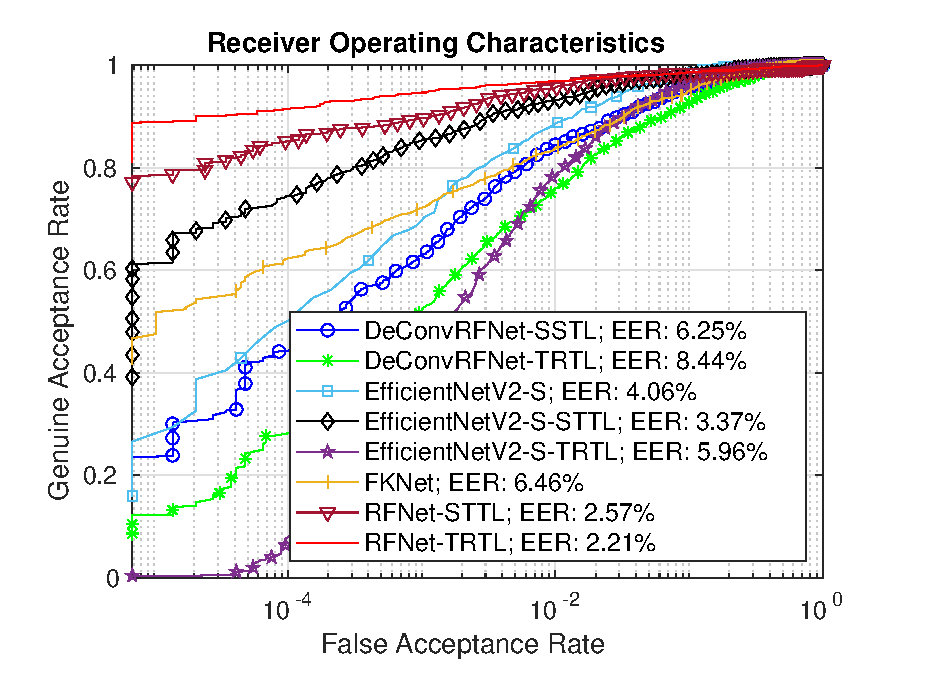
\includegraphics[width=\linewidth]{Figures/fkv3-roc_compare_new.eps}
	\end{subfigure}
	\begin{subfigure}[b]{0.45\linewidth}
		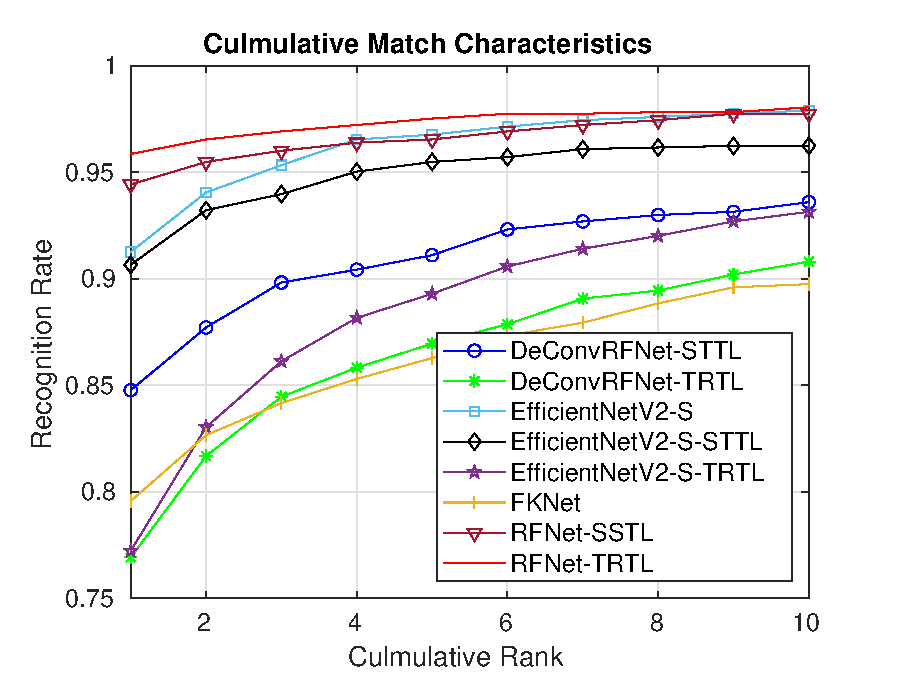
\includegraphics[width=\linewidth]{Figures/fkv3-cmc_compare_new.eps}
	\end{subfigure}
\end{figure}



As for the two-session protocol on the database. I should fine-tune my model on the 105-221 subjects, and use two-session protocol to evaluate my model performance on the 1-104 subjects dataset. In totally, it will generate $104*6=624$ genuine scores, and $104*103*6$ imposter scores. However, the FKNet is a classification task, and the output number classes should be same when training and testing. So the two session protocol experiment is not fit for FKNet. If the FKNet train on the 105-221 subjects and test on the 1-104 subjects with two sessions, the classes is different.

\begin{figure}[H]
    \centering
	\begin{subfigure}[b]{0.45\linewidth}
		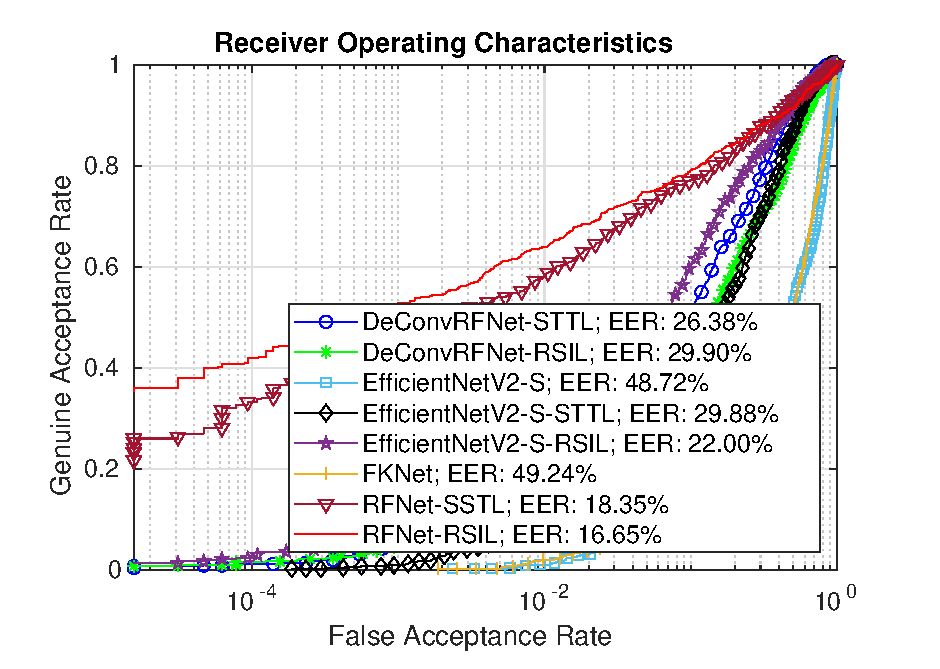
\includegraphics[width=\linewidth]{Figures/two-fkv3roc_compare_new.eps}
	\end{subfigure}
	\begin{subfigure}[b]{0.45\linewidth}
		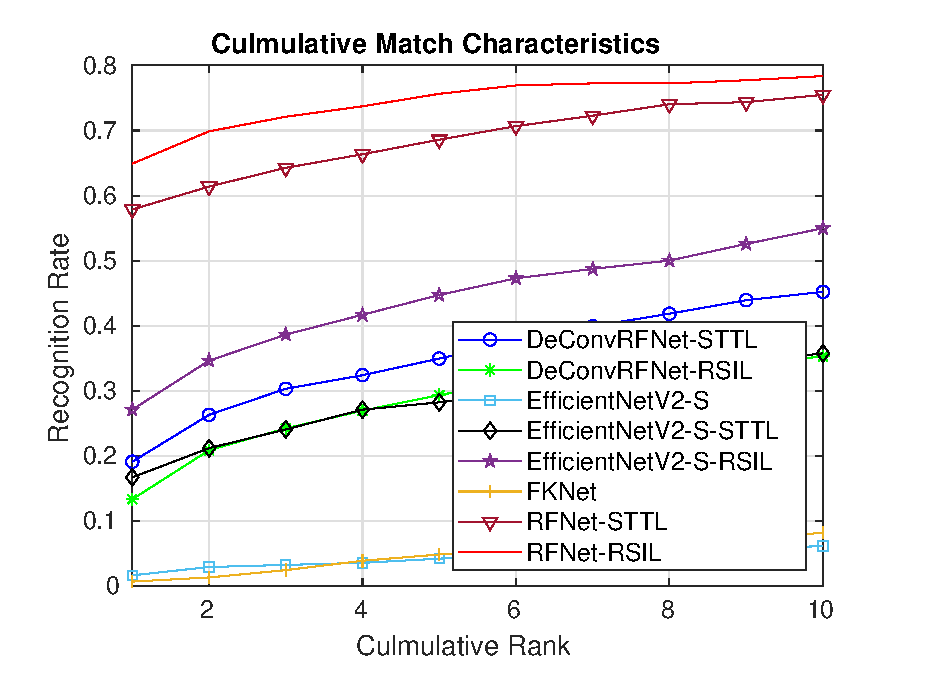
\includegraphics[width=\linewidth]{Figures/two-fkv3cmc_compare_new.eps}
	\end{subfigure}
\end{figure}

The two-session protocol will use the session1 as the probe and use the session2 as the enrollment. As for the genuine matching scores, each sample of a subject will choose the minimal matching score when compare to the rest samples. In this kind of situation, it will have $104x6$ genuine matching scores. Meanwhile, as for the imposter matching scores, it will also choose the minimal value result in $104*103*6$ imposter matching scores on the confusion matrix.

With Yolov5-CSL segmented finger knuckle, the RFNet performance is slightly higher than the local feature descriptors based on key points matching \cite{kumar2020contactless}, and performance higher than the paper \cite{kumar2019toward}. If we want to compare different method performance, I think we should use same dataset. In this kind of situation, the method of \cite{kumar2020contactless} maybe will get higher performance on the segmented finger knuckle by YOLOV5.

\subsubsection{Index Finger Knuckle of Hand Dorsal Image Database}
\begin{figure}[H]
	\centering
	\begin{subfigure}[b]{0.45\linewidth}
		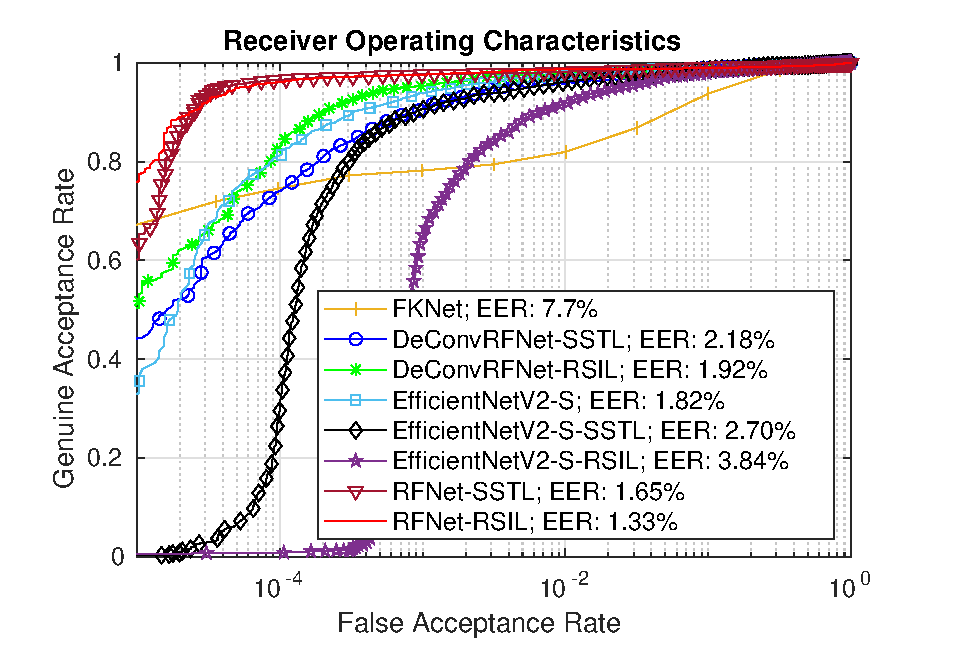
\includegraphics[width=\linewidth]{Figures/hd-roc_compare_new.eps}
	\end{subfigure}
	\begin{subfigure}[b]{0.45\linewidth}
		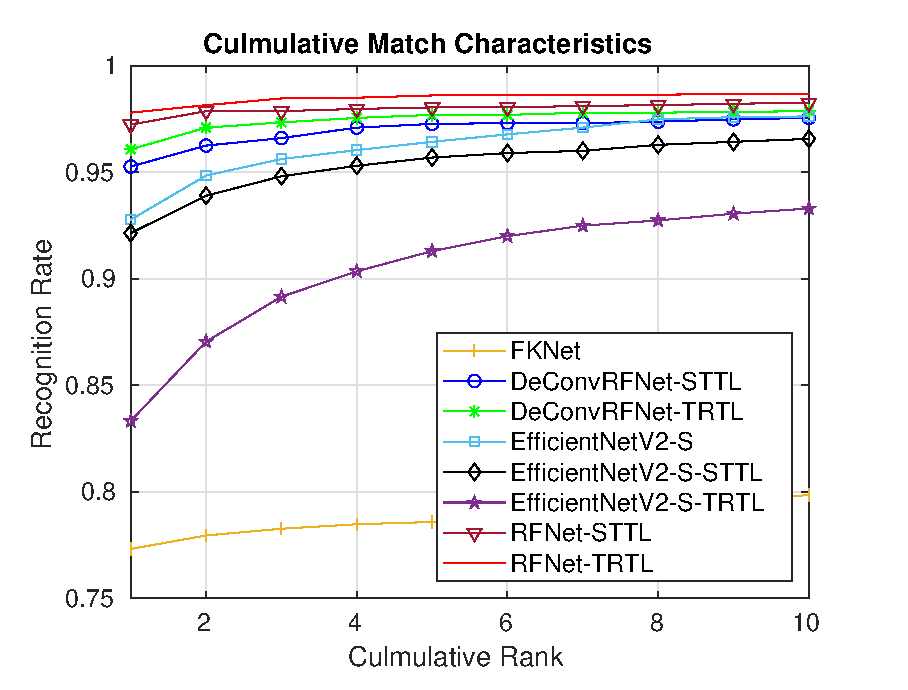
\includegraphics[width=\linewidth]{Figures/hd-cmc_compare_new.eps}
	\end{subfigure}
\end{figure}

As for the experiment, the dataset totally contains 712 subjects, and I use the segmented Index finger knuckle as my dataset. And I fine-tuned my model on the first sample of each subject, and then use the rest four sample as the testing dataset. At the testing process, it has $712*4=2848$ genuine matching scores, and has $712*711*4=2024928$ imposter matching scores. The performance of RFN-128-WRS and RFN-128-WS is similar, but the RFN-128-WS is slightly better than RFN-128-WRS depend on the EER value. And we can get an information that the RFNet is better than the rest network in the ROC figure, including the FKNet.


\subsubsection{2D Samples of 3D Finger Knuckle Database}

First experiment on the database is to use the one session 190 subjects image to fine-tune models and then to test on the another session 190 subjects. It has $190*6$ genuine matching scores and $190*189*6$ imposter matching scores. From the result, we can see that these RFN-128-WRS, RFN-128-WS, EfficientNetV2 can get very high matching accuracy. Meanwhile, the RFNet-TRTL has the minimal EER value among these models. As for the FKNet performance, it gets a very bad result on the 2D images of 3D finger knuckle. I think I have fully trained the FKNet. Maybe the model is overfitting on the training dataset.

\begin{figure}[H]
	\centering
	\begin{subfigure}[b]{0.45\linewidth}
		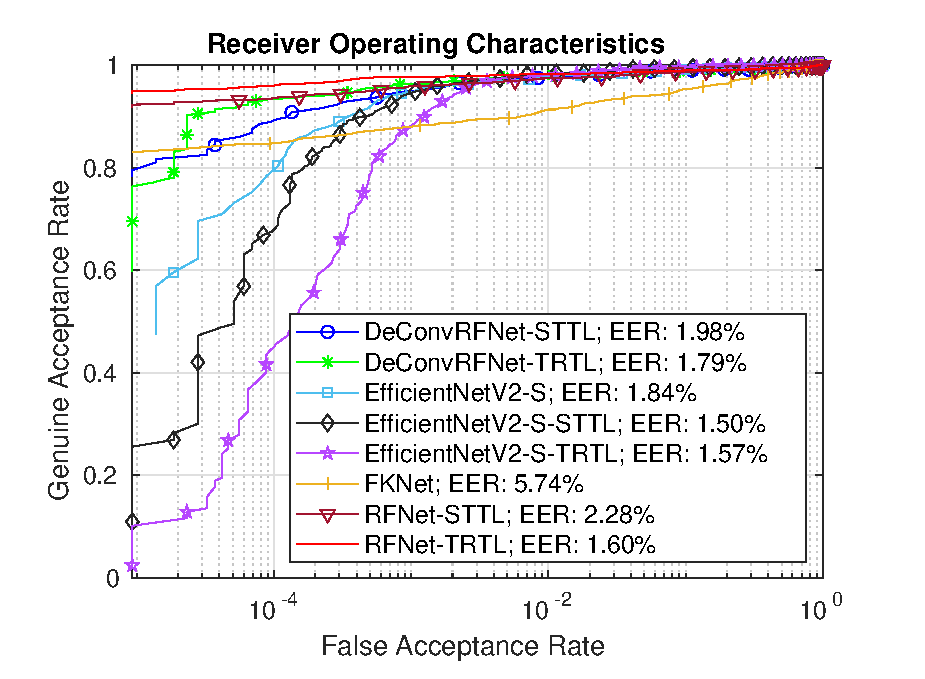
\includegraphics[width=\linewidth]{Figures/2dof3d-roc_compare_new.eps}
	\end{subfigure}
	\begin{subfigure}[b]{0.45\linewidth}
		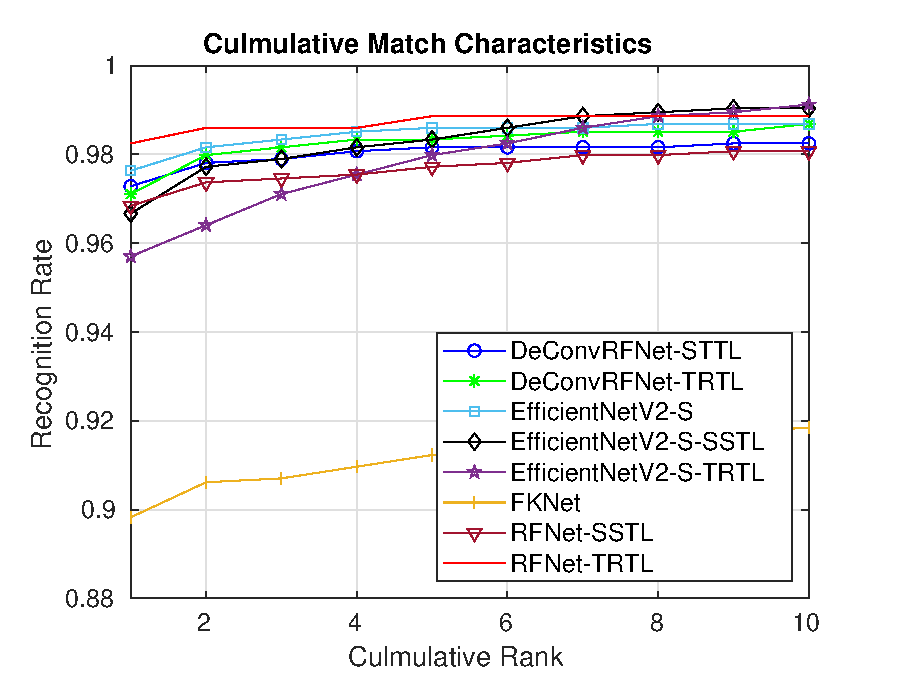
\includegraphics[width=\linewidth]{Figures/2dof3d-cmc_compare_new.eps}
	\end{subfigure}
\end{figure}


And then use the two session protocol. I use the rest samples of session1, and it has 191-228 subjects. In this kind of situation, the training dataset is too small. The two session protocol will test on the 190 subjects, these subjects can offer two session samples. Due to the training set is too small, so the matching performance is not very good. As for the FKNet, it cannot fit on two session protocol due to classification task.

\subsection{Cross Database Performance Evaluation}

From the within database experiment, we can clearly get a conclusion that the RITL loss function can increase the performance compare to the STTL loss function, and the RFNet is better than the DeConvRFNet, EfficientNetV2-S, and FKNet. Meanwhile, the FKNet performance is the worst one. In this section, we will compare these models' performance on the cross database experiment. For these cross database experiment, it can get the generalization ability of neural network, because these data can be regard as unseen data. 

As for the cross database experiment, I firstly pre-trained our models on the Finger Knuckle Images Database V1, and then fine-tuned models on the Finger Knuckle Images Database V3 (with deformation). In the next step, we use our models to test all the finger knuckle of the Hand Dorsal Images Database and the Tsinghua Finger Vein and Finger Dorsal Texture Database (THU-FVFDT3) \cite{thufvfdt3}. Although the THU-FVFDT3 database can offer two-session samples with interval several seconds, but strictly speaking, it is not two-session database. Therefore, I just use the training set of the database (THU-FVFDT-FDT3\_Train) as our evaluation dataset.

\subsubsection{Hand Dorsal Images Database}

\textbf{Index Finger Knuckle and Middle Finger Knuckle}

% \begin{figure}[ht!]
% 	\centering
% 	\begin{subfigure}[b]{0.45\linewidth}
% 		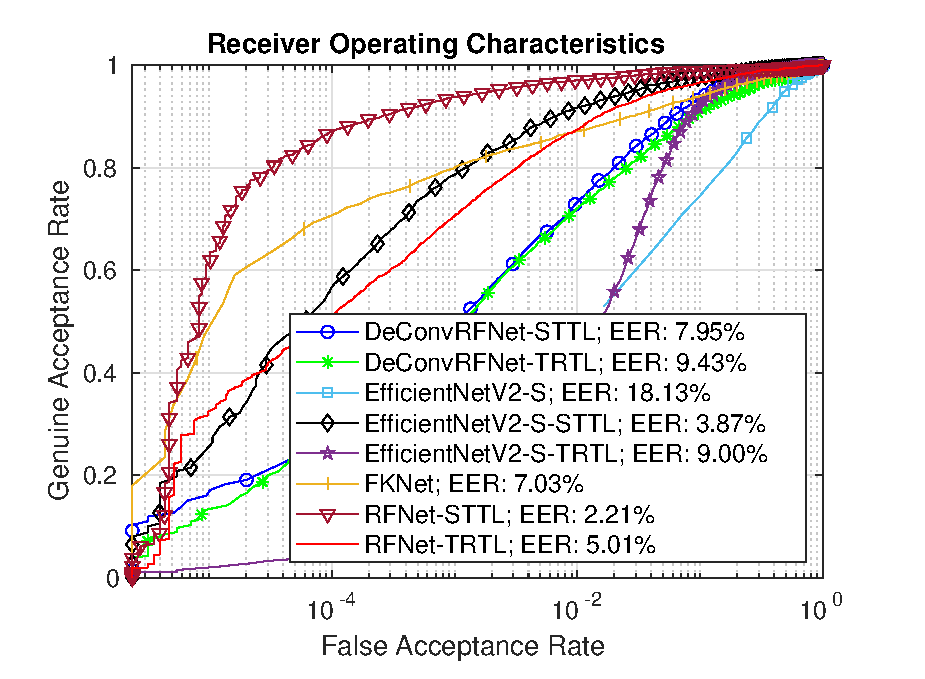
\includegraphics[width=\linewidth]{Figures/crosshd-roc_compare_new.eps}
% 		\caption{}
% 	\end{subfigure}
%     \begin{subfigure}[b]{0.45\linewidth}
% 		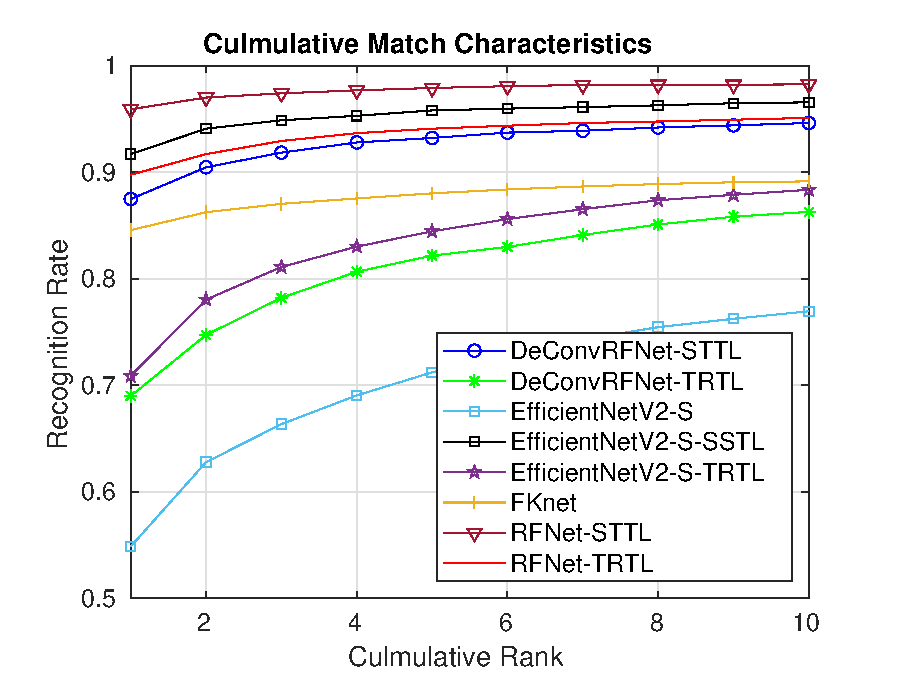
\includegraphics[width=\linewidth]{Figures/crosshd-cmc_compare_new.eps}
% 		\caption{}
% 	\end{subfigure}
% 	\caption{Comparative ROC (a) and corresponding CMC (b) for one-session of the index finger knuckle on the contactless hand dorsal image database \cite{ContactlessHnadDorsaldb}.}
% 	\label{crosshd-index-one-session}
% \end{figure}

% \begin{figure}[ht!]
% 	\centering
% 	\begin{subfigure}[b]{0.45\linewidth}
% 		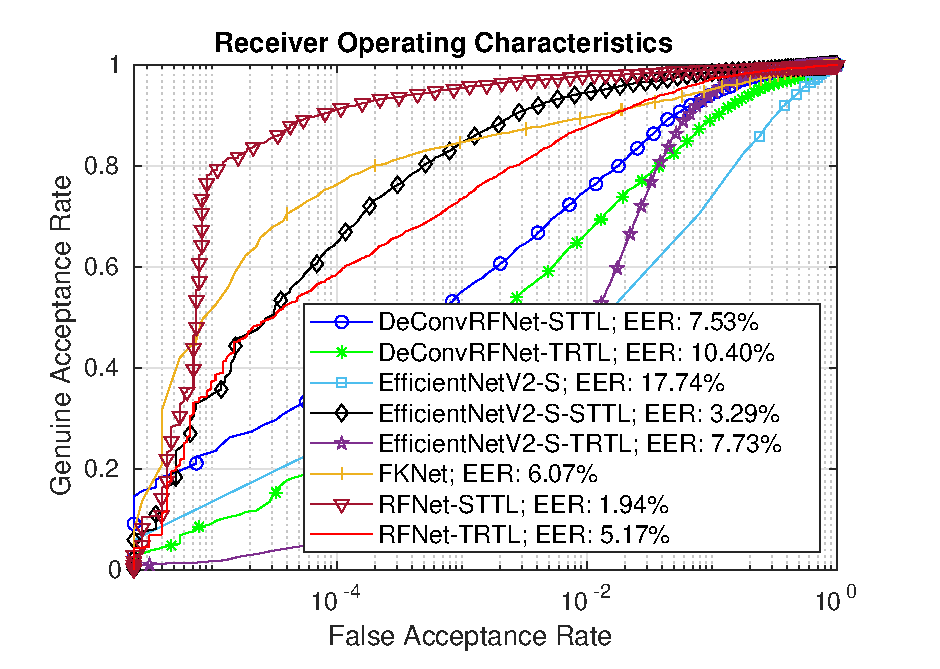
\includegraphics[width=\linewidth]{Figures/crosshd-middle-roc_compare_new.eps}
% 		\caption{}
% 	\end{subfigure}
%     \begin{subfigure}[b]{0.45\linewidth}
% 		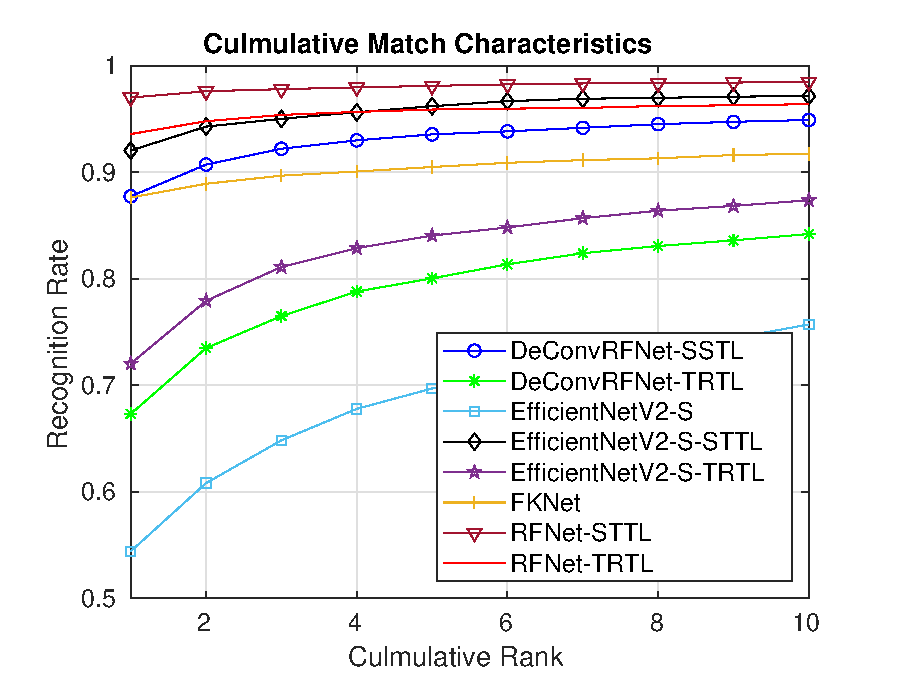
\includegraphics[width=\linewidth]{Figures/crosshd-middle-cmc_compare_new.eps}
% 		\caption{}
% 	\end{subfigure}
% 	\caption{Comparative ROC (a) and corresponding CMC (b) for one-session of the middle finger knuckle on the contactless hand dorsal image database \cite{ContactlessHnadDorsaldb}.}
% 	\label{crosshd-middle-one-session}
% \end{figure}

\begin{figure}[ht!]
	\centering
	\begin{subfigure}[b]{0.45\linewidth}
		\includegraphics[width=\linewidth]{Figures/cross-hd-index-fkv3(yolov5)-105-221/roc_compare_new.eps}
		\caption{}
	\end{subfigure}
    \begin{subfigure}[b]{0.45\linewidth}
		\includegraphics[width=\linewidth]{Figures/cross-hd-index-fkv3(yolov5)-105-221/cmc_compare_new.eps}
		\caption{}
	\end{subfigure}
	\caption{Comparative ROC (a) and corresponding CMC (b) for one-session of the index finger knuckle on the contactless hand dorsal image database \cite{ContactlessHnadDorsaldb}.}
	\label{crosshd-index-one-session}
\end{figure}

The database totally has 712 subjects, and each subject has 5 samples of hand dorsal image. Therefore, it will have $712*5=3560$ genuine matching scores and $712*711*5 = 2531160$ imposter matching scores for index and middle finger knuckle. Figure \ref{crosshd-index-one-session} is the performance result on the index finger.From Figure \ref{crosshd-index-one-session}, all models' cross database performance is similar on the database regardless which finger. We should also notice that STTL is better than RITL on the cross database experiment, while within database, the RITL is better than STTL. It shows that the generalization ability of RITL is not better than STTL to some extent. However, the RFNet-STTL outperform the rest models depend on the ROC and CMC. Even better than FKNet and EfficientNetV2-S, both of them are classification models.



\subsubsection{Tsinghua Finger Vein and Finger Dorsal Texture Database}
\begin{figure}[ht!]
	\centering
	\begin{subfigure}[b]{0.45\linewidth}
		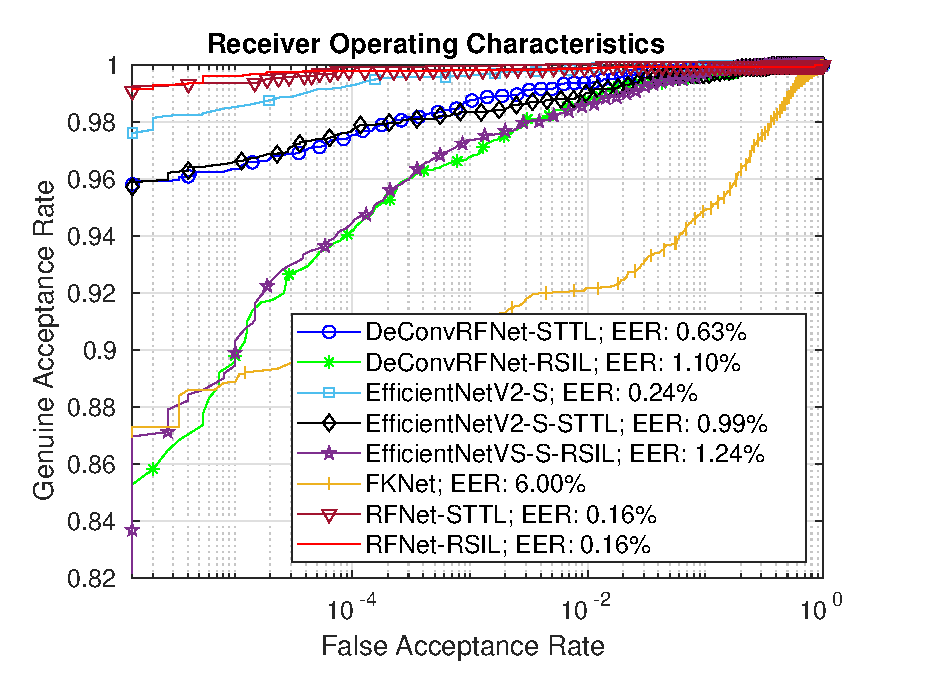
\includegraphics[width=\linewidth]{Figures/crossthu-roc_compare_new.eps}
		\caption{}
	\end{subfigure}
    \begin{subfigure}[b]{0.45\linewidth}
		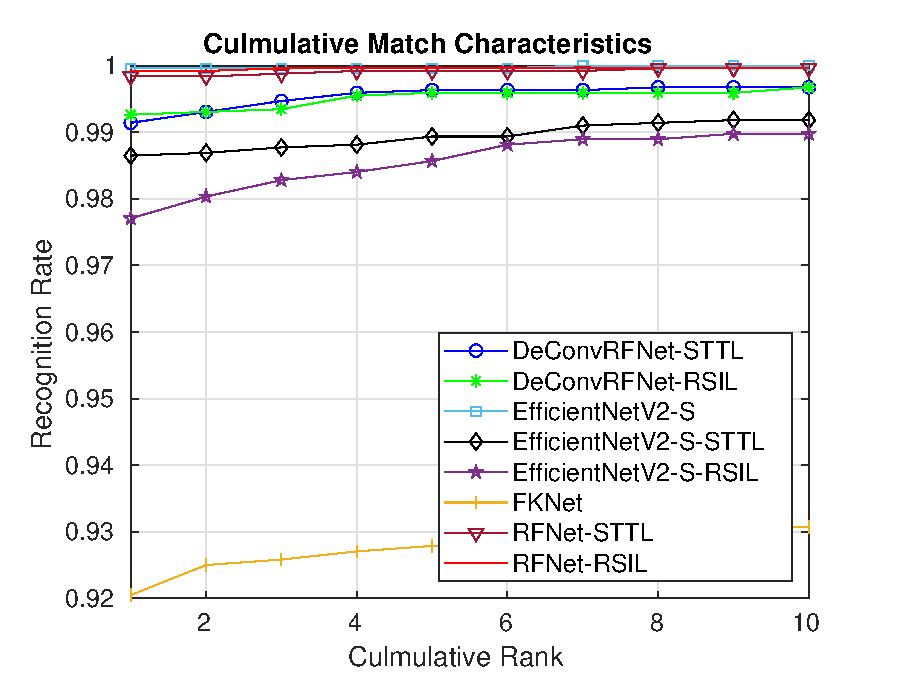
\includegraphics[width=\linewidth]{Figures/crossthu-cmc_compare_new.eps}
		\caption{}
	\end{subfigure}
	\caption{Comparative ROC (a) and corresponding CMC (b) for one-session of the finger dorsal texture images \cite{thufvfdt3}.}
	\label{crossthu-one-session}
\end{figure}

The database \cite{thufvfdt3} has 610 subjects, and each subject can offer 4 samples. From the finger dorsal texture images, we can use our YOLOv5-CSL model to segment finger knuckle images as our testing set. Then as the cross database experiment, it will have $610*4=2440$ genuine matching scores and $610*609*4=1485960$ imposter matching scores. In this database, all models can get very high matching performance from the Figure \ref{crossthu-one-session}, even the worst FKNet can arrive at $6.00\%$ EER on the database. The RFNet with RITL and STTL get the same accuracy, in terms of the CMC, the recognition rate almost arrive at $100\%$.

\subsection{3D Finger Knuckle Images Database}

Because the RFNet with TRTL and STTL can get the best performance on the within database experiment and cross database experiment, 

I have used the matlab code that offered by the FKNet to generate the 3D finger knuckle images for getting the depth information. But it is different that the input image size. The FKNet will resize the original image size $148*212$ to $70*100$ as the testing dataset, and crop from the $70*100$ to $48*80$ as the training dataset. As for RFNet, I just use the original image as the input data. Then the experiment protocol will generate $190*6$ genuine matching scores, and $190*189*6$ imposter matching scores. From the experiment result, we can get that the RFNet is the best model for the 3D Finger Knuckle Database.

\begin{figure}[H]
    \centering
    \begin{subfigure}[b]{0.45\linewidth}
        \includegraphics[width=\linewidth]{Figures/3dod3d-roc_compare_new.eps}
    \end{subfigure}
    \begin{subfigure}[b]{0.45\linewidth}
        \includegraphics[width=\linewidth]{Figures/3dod3d-cmc_compare_new.eps}
    \end{subfigure}
\end{figure}


\subsection{Discussion}
From these experiment results, we can see that EfficientV2-S model is better than FKNet in some dataset. Because EfficientNetV2 model use MBConv as a block unit for replacing residual block. As for MBConv block, it uses depth-wise convolutions to decrease training weights and use Squeeze-Excited block as channel transformer. Meanwhile, the depth of EfficientNetV2-S is deeper than the FKNet.

There is another conclusion is that TRTL generalization ability is lower than STTL loss from the cross database experiment. But in the within database experiment, these model with TRTL loss is better than STTL loss.

..............
\subsection{Ablation Study}

\begin{figure}[ht!]
    \centering
    \begin{subfigure}[b]{0.45\linewidth}
        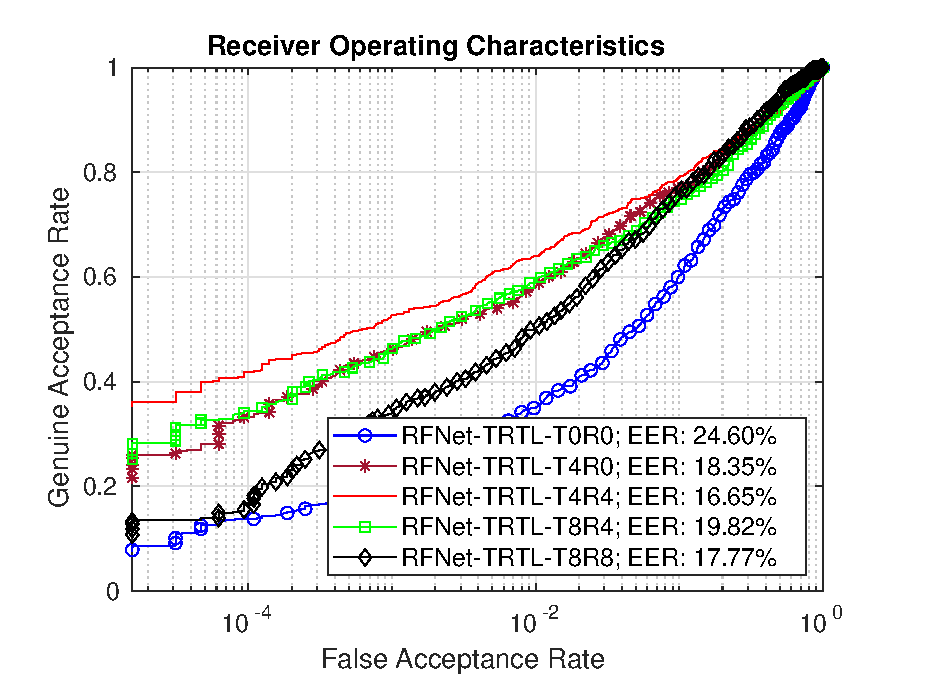
\includegraphics[width=\linewidth]{Figures/ablation-roc_compare_new.eps}
        \caption{}
    \end{subfigure}
    \begin{subfigure}[b]{0.45\linewidth}
        \includegraphics[width=\linewidth]{Figures/ablation-cmc_compare_new.eps}
        \caption{}
    \end{subfigure}
    \caption{Comparative ROC (a) and corresponding CMC (b) for two-session of the 3D finger knuckle database \cite{3dfingerknuckle}.}
    \label{ablation-study}
\end{figure}

.........
\section{Online Contactless Finger Knuckle Identification}

With RSIL loss, the RFNet \cite{liu2020contactless} can outperform state-of-the-art methods. In the previous section, we have estimated its verification and identification performance on different public finger knuckle database, including within-db and cross-db experiments. As for a completely contactless and online finger knuckle identification, the finger knuckle detector is a very important module for automatically detect and segment finger knuckle region. However, as for traditional segmentation algorithm, they cannot correctly segment the finger knuckles in the presence of complex background interference, multiple finger knuckles in the same field of view, obscured finger knuckles or bent finger knuckles.
Meanwhile, as for neural network, the current based on YOLO \cite{redmon2016you}, \cite{redmon2017yolo9000}, \cite{redmon2018yolov3}, \cite{bochkovskiy2020yolov4}, \cite{YOLOv5} and R-CNN \cite{girshick2014rich}, \cite{girshick2015fast}, \cite{ren2015faster}, \cite{he2017mask} series object detection and segmentation approaches cannot simultaneously obtain the angle of finger knuckle and the segmentation with high precision. Especially, the angle of the finger knuckle is a vital factor for identification. If we can get the angle of finger knuckle, we can use angle information to align two feature maps for increasing matching accuracy and efficiency. For solving above problems, we propose rotated bounding box detection based on YOLOv5 model for segmenting and getting angle information.

\subsection{Contactless Finger Knuckle Detection}
\subsubsection{ Oriented Bounding Box Based on YOLOv5}
In order to solve the problem of finger knuckle detection in the real world, we choose to use YOLOv5 model because the YOLO series is famous for its fast detection speed and high accuracy. Especially, the YOLOv5's \cite{YOLOv5} speed can meet our online detection requirements.

\noindent\textbf{Oriented Bounding Box}

\begin{figure}[ht!]
	\centering
	\begin{subfigure}[b]{0.45\linewidth}
		\centering
		\includegraphics[width=0.6\linewidth]{Figures/five-parameter-definition.png}
		\caption{Five-parameter definition with $180^{\circ}$ angular range.}
	\end{subfigure}
	\begin{subfigure}[b]{0.45\linewidth}
		\centering
		\includegraphics[width=0.7\linewidth]{Figures/CSL-angle.png}
		\caption{Circle smooth label with Gaussian window function.}
	\end{subfigure}
	\caption{Oriented rectangle definition and the circle smooth label method.}
\end{figure}


\noindent{However, the YOLOv5 just detect horizontal bounding boxes which cannot offer angle information and will segment a lot of background information. In order to solve these above problem, a rotated bounding box will be predicted instead of horizontal bounding box. As analyzed in this paper \cite{yang2020csl}, the rotated bounding boxes loss will mainly come from angular periodicity and the exchangeability of edges. When use the long side definition of rotated bounding box, it can deal with the exchangeability of edges problem. Meanwhile, using classification task to predict angle can make model easier to train. A periodic coding method called Circular Smooth Label (CSL) \cite{yang2020csl} soft coding can also solve the problem that One-Hot cannot distinguish class relationship. Formula \ref{CSL Function} $g(x)$ is the window function to smooth One-Hot label, and $r$ is a window function of the radius.}

\begin{equation}
    CSL(x)=
    \begin{cases}
        g(x), &\theta-r<x<r+\theta \\
        0   , &\text{otherwise}
    \end{cases}
    \label{CSL Function}
\end{equation}

Furthermore, in this paper, we used the Gaussian function for the Equation \ref{CSL Function} window function, a commonly available function, and used a window radius of 6 to smooth the labels.


\noindent\textbf{Loss function}

\noindent{The original YOLOv5 loss function can have three components. The formula can be simply written as $Loss = CIOU\_Loss + Loss_{obj} + Loss_{class}$. Since the rotated bounding box is based on the modification of YOLOv5, only the angle classification loss is added more. So the total loss function is as expressed in Equation \ref{Loss}, with the addition of $Loss_{angle}$ to YOLOv5 loss function.}
\begin{equation}
    Loss = CIOU\_Loss + Loss_{obj} + Loss_{class} + Loss_{angle}
    \label{Loss}
\end{equation}
\begin{equation}
    \begin{aligned}
        Loss_{angle} = \sum_{i=0}^{S^2}I_{ij}^{obj}\sum_{a{\in}[0,180)}[\hat{P_i(a)}log(P_i(a)) + (1-\hat{P_i(a)})log(1-P_i(a))]
    \end{aligned}
    \label{Loss_angle}
\end{equation}

\subsubsection{Contactless Finger Knuckle Dataset}
Our task is to detect finger knuckles in the contactless and online scenario, but by understanding current public finger knuckle database, their data are collected at specific conditions such as certain angle, certain light. In this kind of situation, this kind of data cannot represent real images of finger knuckle in real world. In order to address the shortcomings of current public finger knuckle dataset for contactless detection, we use a web crawler to get images from the Unsplash \cite{Unsplash} where the keywords are finger knuckles. The Unsplash is an image site that offers uploads and downloads, and uses a copyright license that allows users to download and use them for free or even for commercial use \cite{unsplashlicense}. We have downloaded 2347 images, there are 738 images without knuckles, and these images can be used as background training, and the rest 1609 images that contain at least one finger knuckle are the positive samples for the network model. In the network training process, we use crawled images, 169 finger knuckle images from the HKPolyU Finger Knuckle Database (V1.0) \cite{fingerknuckledbv1.0}, and 64 finger knuckles images from the HKPolyU Hand Dorsal Database \cite{ContactlessHnadDorsaldb} as for the training set. And we use the rest data as testing set to evaluate performance. The most important part is the data augmentation which contains flip, rotation, resize, translate and mosaic.

\subsubsection{Contactless Finger Knuckle Detection}

\noindent\textbf{Detection Performance}

\noindent
The YOLOv4, YOLOv5x, and YOLOv5m model predict horizontal bounding box, while the remaining YOLOv5 model predict oriented bounding box with CSL classification, called YOLOv5-CSL. We can see the performance difference between these variations of the YOLOv5 model from the Table \ref{mAP of different model}. Among the downloaded 2580 images, 100 images were randomly selected as the testing set. 

\begin{table}[ht!]
    \centering
    \begin{tabular}{c c c c c c}
        \hline
        Model & \makecell[c]{Total \\ Time/ms\\ (1024x1024)} & \makecell[c]{Number \\of Layers} & \makecell[c]{${mAP}^{val}$\\0.5} & \makecell[c]{AP of\\ Major \\FK} & \makecell[c]{AP of\\ Minor \\FK}\\
        \hline
        YOLOv5x-CSL & 40.9 & 407 & \textbf{89.9} &\textbf{89.6} & \textbf{90.1} \\
        YOLOv5m-CSL & 23.3 & 263 & 85.7 & 88.9 & 80.4 \\
        YOLOv5x & 33.3 ms & 407 & 87.3 & 86.5 & 88.0  \\
        YOLOv5m & 12.1ms & 263 & 84.8 & 84.5 & 85.1 \\
        \hline
    \end{tabular}
    \caption{Comparison of the accuracy of the different models of the YOLO series for detecting finger knuckle. The calculated values of mAP were measured at a detection threshold of 0.001 as well as an IOU threshold of 0.5. All the experiments are test on the GTX 2080 GPU and I7-7800X CPU, and the total time includes the inference and NMS process.}
    \label{mAP of different model}
\end{table}

\textbf{Segmentation Performance}

This section aim to compare quality of finger knuckle between YOLOv5-CSL segmented and dataset offered. Because the segmented finger knuckle on the 3D Finger Knuckle Dataset already have high quality, I mainly test on the Index Finger Knuckle of Hand Dorsal Dataset and the Finger Knuckle Dataset V3 (with deformable).

\begin{figure}[H]
	\centering
	\begin{subfigure}[b]{0.45\linewidth}
		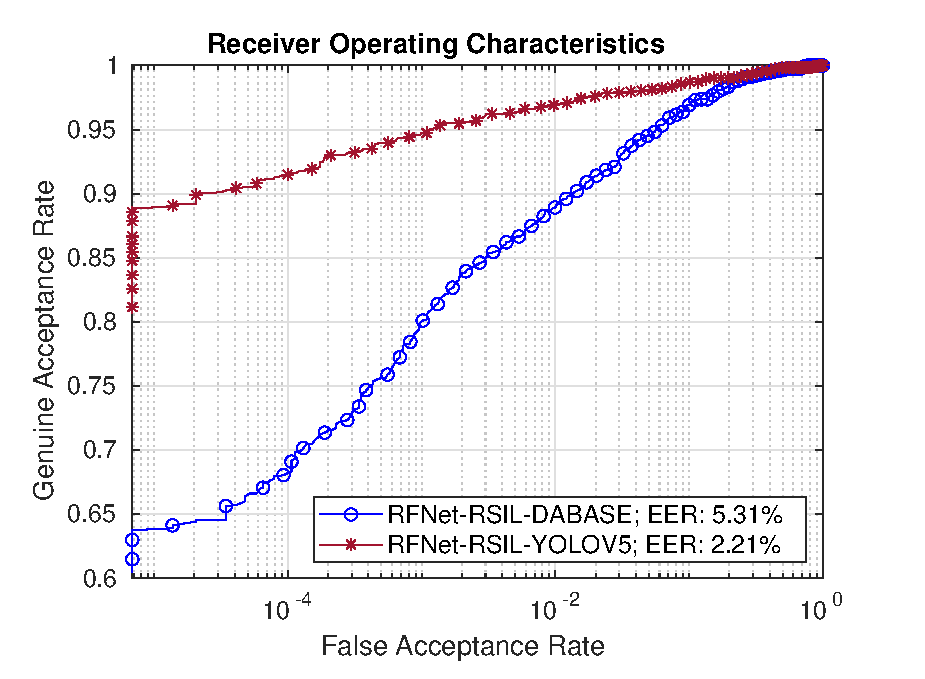
\includegraphics[width=\linewidth]{Figures/yolov5vsdatabase/fkv3-roc_compare_new.eps}
	\end{subfigure}
	\begin{subfigure}[b]{0.45\linewidth}
		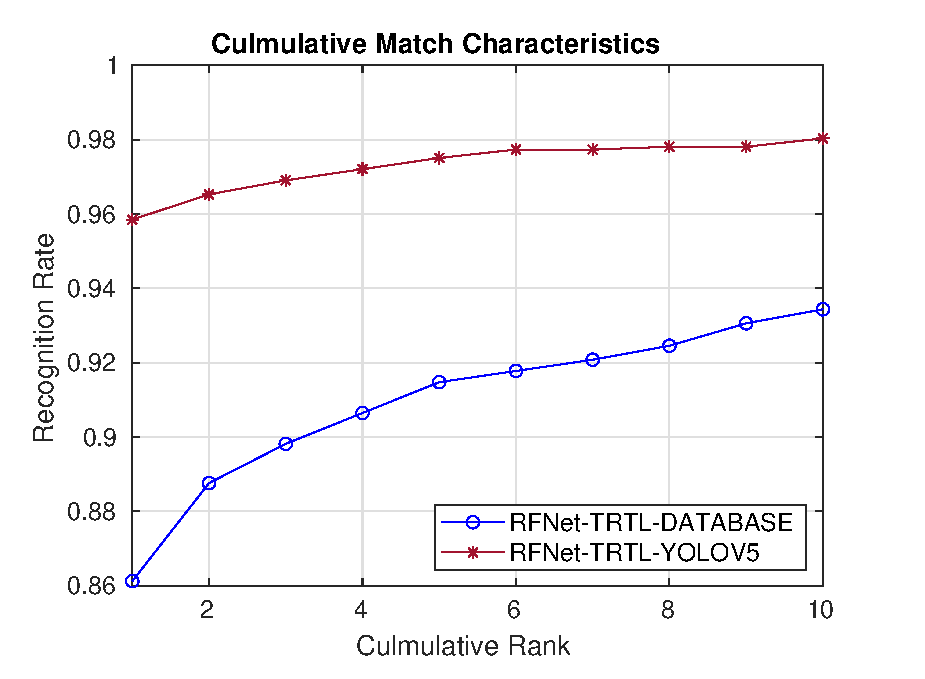
\includegraphics[width=\linewidth]{Figures/yolov5vsdatabase/fkv3-cmc_compare_new.eps}
	\end{subfigure}
	\caption{Compare performance on the Finger Knuckle V3 Dataset (with deformable)}
\end{figure}

\begin{figure}[H]
	\centering
	\begin{subfigure}[b]{0.45\linewidth}
		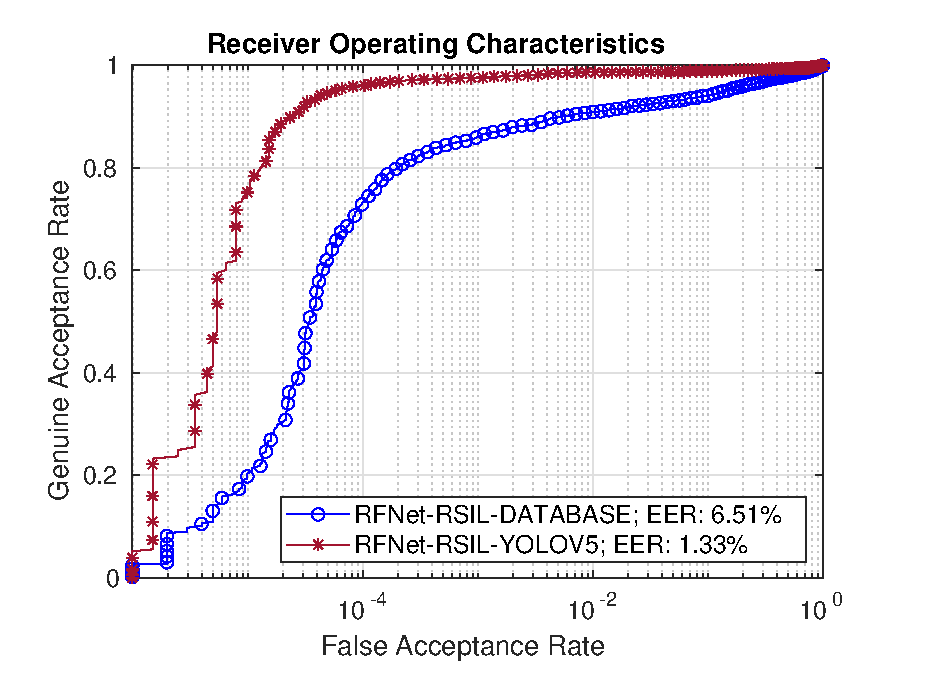
\includegraphics[width=\linewidth]{Figures/yolov5vsdatabase/hd-roc_compare_new.eps}
	\end{subfigure}
	\begin{subfigure}[b]{0.45\linewidth}
		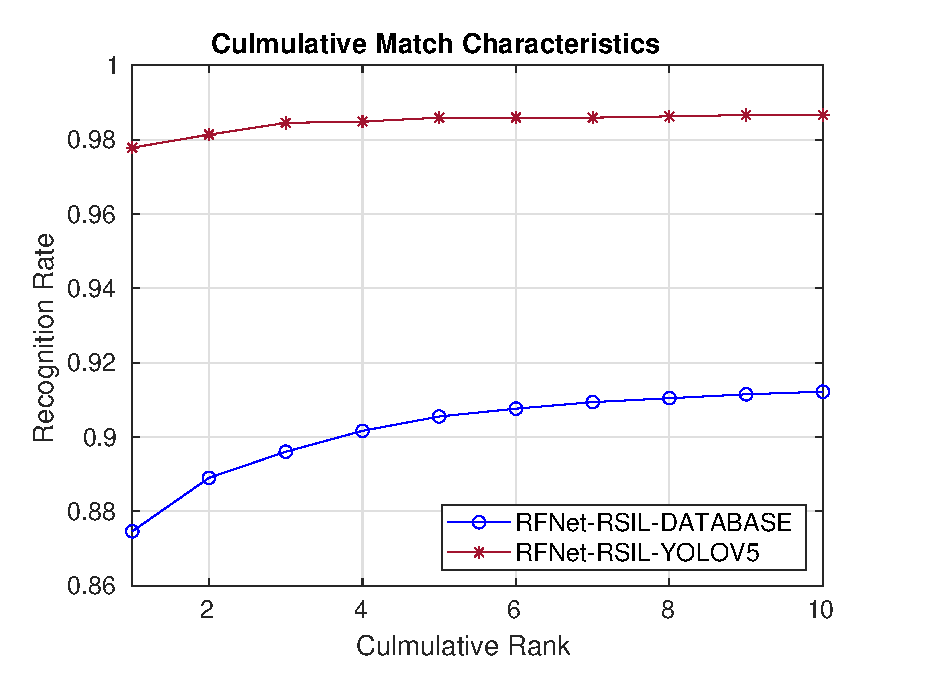
\includegraphics[width=\linewidth]{Figures/yolov5vsdatabase/hd-cmc_compare_new.eps}
	\end{subfigure}
	\caption{Compare performance on the Index Finger of the Hand Dorsal Image Database.}
\end{figure}

From the above figures, we can clearly get the conclusion that quality of segmented finger knuckle of YOLOv5 is better than the segmented finger knuckle of dataset through the ROC curve and CMC curve. Especially on the Hand Dorsal Image Database, the EER value can drop from $6.51\%$ to $1.33\%$. 



 \subsection{Online Contactless Finger Knuckle Identification Performance}

 For proving our contactless and online finger knuckle identification performance, we capture  52 subjects and each subject can offer about 15-20s contactless finger knuckle video. The minimum frame rate of the videos we offer is 30 frames per second. We choose two method to get the contactless finger knuckle images, one is that we get 1 image per second, another one is that we get 6 images per second for testing online matching performance. Because the shortest video is 15s, for 1 image per second, we can totally get $52*15 = 780$ finger knuckle images for keeping the same number of samples result in $52*15 =1789 $ genuine matching scores and $52*51*15 = 39780$ imposter matching scores. In terms of the 6 images per second, we can get $52*15*6=4680$ finger knuckle samples, result in $52*90=4680$ genuine matching scores and $52*51*90=238680$ imposter matching scores.
 .............

 \begin{figure}[H]
	\centering
	\begin{subfigure}[b]{0.45\linewidth}
		\includegraphics[width=\linewidth]{Figures/online-performance/1s1f-roc_compare_new.eps}
		\caption{}
	\end{subfigure}
	\begin{subfigure}[b]{0.45\linewidth}
		\includegraphics[width=\linewidth]{Figures/online-performance/1s1f-cmc_compare_new.eps}
		\caption{}
	\end{subfigure}
	\caption{Comparative ROC (a) and corresponding CMC (b) with one session protocol for }
\end{figure}

\begin{figure}[H]
	\centering
	\begin{subfigure}[b]{0.45\linewidth}
		\includegraphics[width=\linewidth]{Figures/online-performance/1s6f-roc_compare_new.eps}
	\end{subfigure}
	\begin{subfigure}[b]{0.45\linewidth}
		\includegraphics[width=\linewidth]{Figures/online-performance/1s6f-cmc_compare_new.eps}
	\end{subfigure}
	\caption{}
\end{figure}
\section{Conclusions and Future Work}

The generalization performance of convolutional neural networks is extremely powerful, and the features extracted by the convolutional kernel are so robust, for example with scale invariance, that neural networks have started to replace traditional feature description operators. However, neural networks do not have capabilities such as rotation invariance and translation invariance \cite{jaderberg2015spatial}. In practical application scenarios, contactless finger knuckle recognition system, are most susceptible to problems such as interference from complex backgrounds, and affine transformation such as rotation or translation of finger knuckle. Therefore, we propose the RSIL loss for increase the neural network rotating and shifting invariance performance. From the within database and cross database matching performance on the experiment section, it shows that with our RSIL loss, RFNet-RSIL can outperform state-of-the-art on the listed public finger knuckle database. We have also based the YOLOv5 model to resolve the interference of complex backgrounds and to obtain angular information to further mitigate the rotation problem. In Section 5, YOLOv5x-CSL can get a high mAP value on finger knuckle detection, and using it for segmenting finger knuckle can improve the matching accuracy.

Since we have design a completely contactless and online finger knuckle identification system, but we still have to solve several limitations. The first problem is the amount of data. For practical applications in various industries, the current amount of data on the finger knuckle is too sparse to allow the model to be adequately trained, unlike face recognition and fingerprint recognition which have such a large amount of data. To further improve performance is to increase the amount of data on the finger knuckle. Not only are the finger knuckle prone to rotation and translation, but an even greater headache is the problem of deformation, which occurs even in 3D space. In the deformable finger knuckle database \cite{fingerknuckledbv3.0}, our method performance not very good. This is because the finger knuckle are partially flexible. Even though I used deformable convolution, it did not improve the matching performance. We think a future direction could deal with chunked feature maps or first extracting key points, such as ending points or bifurcation, and then getting a local match based on the location of these key points. Another problem is that our current approach is two-stage, where a network is trained to detect the position of the finger knuckle in order to segment. Then, another network is used to extract the finger knuckle features for matching. In fact, the finger knuckle features are already extracted during finger knuckle detection, therefore, why not use it to indirectly match the finger knuckle as an end-to-end model. Or do multitask model instead of such a tedious process.

\input{references.tex}

\end{document}
